%\documentclass[a4paper,landscape]{article}
\documentclass[12pt]{amsart}

\usepackage{fullpage}
\usepackage{amscd,amsfonts,amsmath,amssymb,amstext,amsthm}
\usepackage[mathscr]{euscript}
\usepackage{amsrefs}
\usepackage{enumerate}
\usepackage{verbatim}
\usepackage{graphicx}
\usepackage{tikz}
\usepackage{pgfplots}
\pgfplotsset{compat=1.15}
\usepackage{mathrsfs}
\usetikzlibrary{arrows}
\usepackage{comment}
%\pagenumbering{gobble}
% % % % % % % % % % 

\newcommand{\C}{\mathbb C} 
\newcommand{\Z}{\mathbb Z}
\newcommand{\vect}[1]{\mathbf{#1}}
\newcommand{\N}{\mathbb N}
\newcommand{\R}{\mathbb R}
\newcommand{\tns}{\otimes}
\newcommand{\Prj}{\mathbb P}
\DeclareMathOperator{\rank}{rank}
\DeclareMathOperator{\rref}{rref}
\DeclareMathOperator{\Span}{span}
\DeclareMathOperator{\Spec}{Spec}
\DeclareMathOperator{\Cone}{Cone}
\DeclareMathOperator{\Conv}{Conv}
\DeclareMathOperator{\Hom}{Hom}
\DeclareMathOperator{\Relint}{Relint}
\DeclareMathOperator{\Star}{Star}
\DeclareMathOperator{\Bl}{Bl}
\DeclareMathOperator{\Div}{Div}
\DeclareMathOperator{\Cl}{Cl}
\DeclareMathOperator{\divv}{div}
\DeclareMathOperator{\Pic}{Pic}
\DeclareMathOperator{\SF}{SF}
\DeclareMathOperator{\CDiv}{CDiv}
\DeclareMathOperator{\argmax}{argmax}
\DeclareMathOperator{\coker}{coker}
%%%%%%%%%%%%%%%%%%%%%%%%%%%%%%%%%%%%%%%%%
\theoremstyle{plain}
\newtheorem{thm}{Theorem}[subsection]
\newtheorem{prop}[thm]{Proposition}
\newtheorem{lem}[thm]{Lemma}
\newtheorem{cor}{Corollary}[thm]

\theoremstyle{definition}
\newtheorem{dfn}[thm]{Definition}
\newtheorem{ex}[thm]{Example}
\newtheorem*{exe*}{Exercise}

\theoremstyle{remark}
\newtheorem{rmk}[thm]{Remark}
%%%%%%%%%%%%%%%%%%%%%%%%%%%%%%%%%%%%%%%%

\title{Results}
\date{\today}

\begin{document}
\maketitle

\section{Generating set for $\sigma$}
Let $\vect e_{11}, \vect e_{12},\dots, \vect e_{1n}, \vect e_{22}, \vect e_{23}, \dots, \vect e_{nn}$ be a basis for $\mathbb{Z}^{\binom{n+1}{2}}$. We have $\sigma^\vee = \Cone(\mathscr{A})$ for $\mathscr{A} = \{\vect e_{ij}, \vect e_{ii} - \vect e_{ij} + \vect e_{jj}\mid i\leq j\}$.

Claim: For $\sigma$ as above, we have \[\sigma = (\sigma^\vee)^\vee = \Cone(\mathscr{B}).\] for \begin{multline*}
    \mathscr{B} = \{\vect e_{ii}, \vect e_{ii} + \vect e_{ij_1} + \cdots + \vect e_{ij_r} + \vect e_{j^\prime_1i} + \cdots + \vect e_{j^\prime_{r^\prime}i}\mid \\ 1\leq i\leq n,~ r,r^\prime >0,~ j_h>i \text{ for } 1\leq h \leq r,~ j^\prime_{h^\prime}< i\text{ for } 1\leq h^\prime\leq r^\prime\}
\end{multline*}
\begin{proof}
    Given $u = (b_{11},\dots,b_{1n},b_{22},\dots,b_{2n},\dots,b_{nn})\in N_{\mathbb{R}}\cong \mathbb{R}^{\binom{n+1}{2}}$, we have that $u\in\sigma$ if and only if: \begin{enumerate}
        \item $b_{ij}\geq 0$, for all $i\leq j$
        \item $b_{ii}-b_{ij}+b_{jj}\geq 0$, for all $ i< j$
    \end{enumerate}
    This follows from the definition of the dual cone. The vector $u$ is in $\sigma$ if and only if $\langle u,a\rangle \geq 0$ for any $a\in \sigma^\vee$. In particular, $\langle u,a\rangle \geq 0$ for $a\in \{\vect e_{ii}, \vect e_{ii} - \vect e_{ij} + \vect e_{jj}\mid i\leq j\} = \mathscr{A}$, which gives the above inequalities. 


    It is clear that $\sigma^\prime = \Cone(\mathscr{B})$ is contained in $\sigma$. (The inner product is bilinear so it suffices to see that the inner product of any generator of $\sigma^\prime$ with any generator of $\sigma^\vee$ is nonnegative.)

    To show that $\sigma\subseteq \sigma^\prime$, we show instead that elements not in $\sigma^\prime$ are not in $\sigma$.
    
    An element not in $\Cone(\mathscr{B})$ is given by a linear combination $\sum_{p=1}^q b_p\beta_p$ for $\beta_p\in \mathscr{B}$ where at least one $b_p$ is negative. As a result we see that $\vect e_{ij_h}, \vect e_{j_h^{\prime}i}$ are not in $\Cone(\mathscr{B})$ for $1\leq i\leq n,~ r,r^\prime >0,~ j_h>i \text{ for } 1\leq h \leq r,~ j^\prime_{h^\prime}< i\text{ for } 1\leq h^\prime\leq r^\prime$. 

    Hence we can decompose any element $u^{\prime}$ not in $\Cone(\mathscr{B})$ into a sum of the following form: \begin{multline*}
        u^{\prime} = \sum_{g = 1}^{r^{\prime\prime\prime}}  \big[ b_{i_gi_g}\vect e_{i_gi_g} +  b_{i_gj_1}\vect e_{i_gj_1} +\cdots + b_{i_gj_r}\vect e_{i_gj_r} + b_{j^{\prime}_1i_g}\vect e_{j^{\prime}_1i_g} +\cdots + b_{j^{\prime}_{r^{\prime}}i_g}\vect e_{j^{\prime}_{r^{\prime}}i_g} \\  + b_{k_1\ell_1}\vect e_{k_1\ell_1} +\cdots + b_{k_{r^{\prime\prime}}\ell_{r^{\prime\prime}}}\vect e_{k_{r^{\prime\prime}}\ell_{r^{\prime\prime}}} \big]
    \end{multline*} where $1\leq i\leq n,~ r,r^\prime,r^{\prime\prime}, r^{\prime\prime\prime} >0,~ j_h>i$ for $1\leq h \leq r,~ j^\prime_{h^\prime}< i$ for $1\leq h^\prime\leq r^\prime$ and $b_{k_{h^{\prime\prime}}\ell_{h^{\prime\prime}}} \neq 0 , k_{h^{\prime\prime}}\neq \ell_{h^{\prime\prime}}\neq i$ for $1\leq h^{\prime\prime}\leq r^{\prime\prime}$. But $u^{\prime}$ cannot be in $\sigma$ as it violates condition (2) above.

    Hence elements not in $\sigma^\prime$ are not in $\sigma$, so the reverse inclusion holds and $\sigma = \sigma^\prime$.
\end{proof}
\newpage

    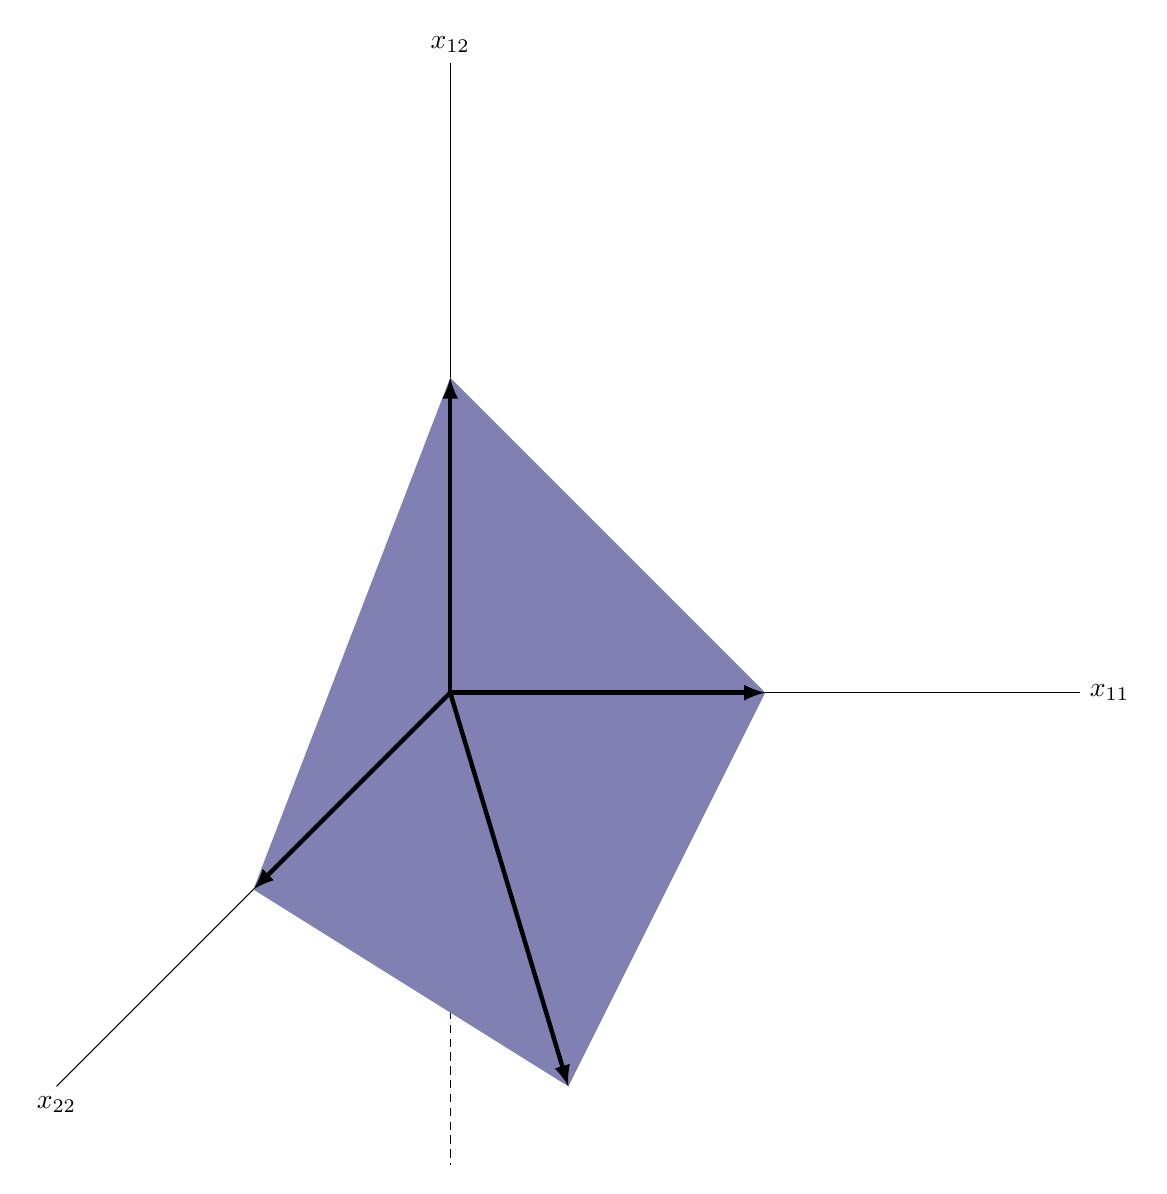
\begin{tikzpicture}[>=latex]
        \draw (0,0) -- (0,8) node [above, black] {$x_{12}$};
        \draw[densely dashed] (0,0) -- (0,-6);
        \draw (0,0) -- (8,0) node [right, black] {$x_{11}$};
        \draw (0,0) -- (-5,-5) node [below, black] {$x_{22}$};

        \fill[blue!40!black!50!white] (0,0) -- (4,0) -- (0,4);
        \fill[blue!40!black!50!white] (0,0) -- (-2.5,-2.5) -- (0,4);
        \fill[blue!40!black!50!white] (0,0) -- (-2.5,-2.5) -- (1.5,-5);
        \fill[blue!40!black!50!white] (0,0) -- (4,0) -- (1.5,-5);

        \draw [->,ultra thick] (0,0) -- (4,0); 
        \draw [->,ultra thick] (0,0) -- (0,4); 
        \draw [->,ultra thick] (0,0) -- (-2.5,-2.5); 
        \draw [->,ultra thick] (0,0) -- (1.5,-5); 
    \end{tikzpicture}

    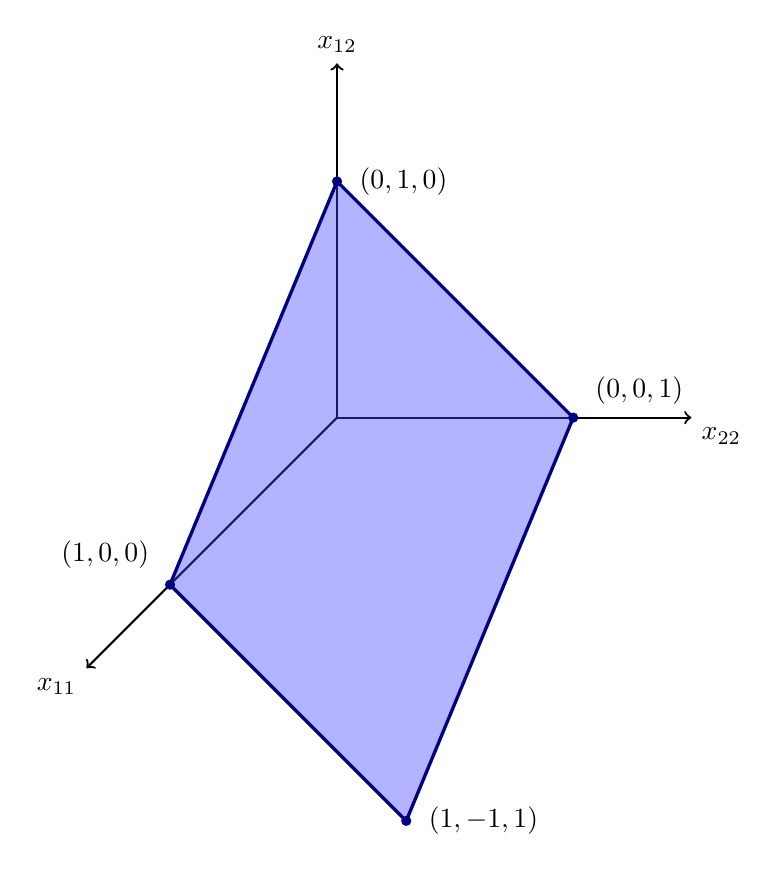
\begin{tikzpicture}%
        [x={(-0.707106cm, -0.707106cm)},
        y={(1cm, 0cm)},
        z={(0cm, 1cm)},
        scale=3.000000,
        back/.style={loosely dotted, thin},
        edge/.style={color=blue!50!black, very thick},
        facet/.style={fill=blue!75!white,fill opacity=0.400000},
        vertex/.style={inner sep=1pt,circle,draw=blue!50!black,fill=blue!50!black,thick}]
    %
    %
    %% This TikZ-picture was produced with Sagemath version 9.6
    %% with the command: ._tikz_2d_in_3d and parameters:
    %% view = [-0.124500000000000, -0.300500000000000, -0.945600000000000]
    %% angle = 145
    %% scale = 2
    %% edge_color = orange
    %% facet_color = orange
    %% opacity = 0.400000000000000
    %% vertex_color = blue
    %% axis = True
    
    %% Drawing the axes
    \draw[color=black,thick,->] (0,0,0) -- (1.5,0,0) node[anchor=north east]{$x_{11}$};
    \draw[color=black,thick,->] (0,0,0) -- (0,1.5,0) node[anchor=north west]{$x_{22}$};
    \draw[color=black,thick,->] (0,0,0) -- (0,0,1.5) node[anchor=south]{$x_{12}$};
    %% Coordinate of the vertices:
    %%
    \coordinate (0.00000, 0.00000, 1.00000) at (0.00000, 0.00000, 1.00000);
    \coordinate (0.00000, 1.00000, 0.00000) at (0.00000, 1.00000, 0.00000);
    \coordinate (1.00000, 0.00000, 0.00000) at (1.00000, 0.00000, 0.00000);
    \coordinate (1.00000, 1.00000, -1.00000) at (1.00000, 1.00000, -1.00000);
    %%
    %%
    %% Drawing the interior
    %%
    \fill[facet] (1.00000, 1.00000, -1.00000) -- (0.00000, 1.00000, 0.00000) -- (0.00000, 0.00000, 1.00000) -- (1.00000, 0.00000, 0.00000) -- cycle {};
    %%
    %%
    %% Drawing edges
    %%
    \draw[edge] (0.00000, 0.00000, 1.00000) -- (0.00000, 1.00000, 0.00000);
    \draw[edge] (0.00000, 0.00000, 1.00000) -- (1.00000, 0.00000, 0.00000);
    \draw[edge] (0.00000, 1.00000, 0.00000) -- (1.00000, 1.00000, -1.00000);
    \draw[edge] (1.00000, 0.00000, 0.00000) -- (1.00000, 1.00000, -1.00000);
    %%
    %%
    %% Drawing the vertices
    %%
    \node[vertex,label={[label distance=0.1cm]0:$(0,1,0)$}] at (0.00000, 0.00000, 1.00000)    {};
    \node[vertex,label={[label distance=0.1cm]15:$(0,0,1)$}] at (0.00000, 1.00000, 0.00000)     {};
    \node[vertex,label={[label distance=0.1cm]150:$(1,0,0)$}] at (1.00000, 0.00000, 0.00000)     {};
    \node[vertex,label={[label distance=0.1cm]0:$(1,-1,1)$}] at (1.00000, 1.00000, -1.00000)     {};
    %%
    %%
    \end{tikzpicture}

    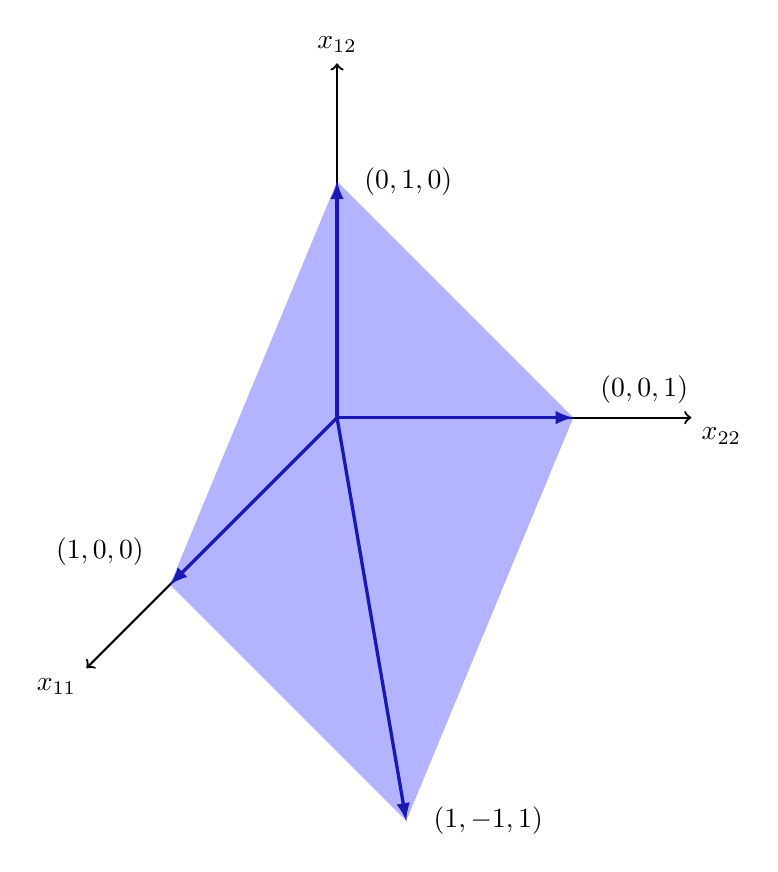
\begin{tikzpicture}%
        [x={(-0.707106cm, -0.707106cm)},
        y={(1cm, 0cm)},
        z={(0cm, 1cm)},
        scale=3.000000,
        back/.style={loosely dotted, thin},
        edge/.style={color=blue!50!black, very thick},
        facet/.style={fill=blue!75!white,fill opacity=0.400000},
        facet2/.style={fill=blue!75!black,fill opacity=0.400000},
        vertex/.style={inner sep=1pt,circle,draw=blue!50!black,fill=blue!50!black,thick}]

    %% Drawing the axes
    \draw[color=black,thick,->] (0,0,0) -- (1.5,0,0) node[anchor=north east]{$x_{11}$};
    \draw[color=black,thick,->] (0,0,0) -- (0,1.5,0) node[anchor=north west]{$x_{22}$};
    \draw[color=black,thick,->] (0,0,0) -- (0,0,1.5) node[anchor=south]{$x_{12}$};
    %% Rays for cone:   
    \draw[color=blue!50!black,very thick,-latex] (0,0,0)--(0,0,1);
    \draw[color=blue!50!black,very thick,-latex] (0,0,0)--(0,1,0);
    \draw[color=blue!50!black,very thick,-latex] (0,0,0)--(1,0,0);
    \draw[color=blue!50!black,very thick,-latex] (0,0,0)--(1,1,-1);
    %% Coordinate of the vertices:
    %%
    \coordinate (0.00000, 0.00000, 1.00000) at (0.00000, 0.00000, 1.00000);
    \coordinate (0.00000, 1.00000, 0.00000) at (0.00000, 1.00000, 0.00000);
    \coordinate (1.00000, 0.00000, 0.00000) at (1.00000, 0.00000, 0.00000);
    \coordinate (1.00000, 1.00000, -1.00000) at (1.00000, 1.00000, -1.00000);
    %%
    %%
    %% Drawing the interior
    %%
    \fill[facet] (0, 0, 0) -- (0, 1, 0) -- (0, 0, 1) -- (0, 0, 0) -- cycle {};
    \fill[facet] (0,0,0) -- (1, 1, -1) -- (0, 1, 0) -- (0, 0, 0) -- cycle {};
    \fill[facet] (0,0,0) -- (1,0,0) -- (1, 1, -1) -- (0, 0, 0) -- cycle {};
    \fill[facet] (0, 0, 0) -- (1, 0, 0) -- (0, 0, 1) -- (0, 0, 0) -- cycle {};
    %%
    %% Drawing the vertices
    %%
    \node[label={[label distance=0.1cm]0:$(0,1,0)$}] at (0.00000, 0.00000, 1.00000)    {};
    \node[label={[label distance=0.1cm]15:$(0,0,1)$}] at (0.00000, 1.00000, 0.00000)     {};
    \node[label={[label distance=0.1cm]150:$(1,0,0)$}] at (1.00000, 0.00000, 0.00000)     {};
    \node[label={[label distance=0.1cm]0:$(1,-1,1)$}] at (1.00000, 1.00000, -1.00000)     {};
    %%
    %%
    \end{tikzpicture}

    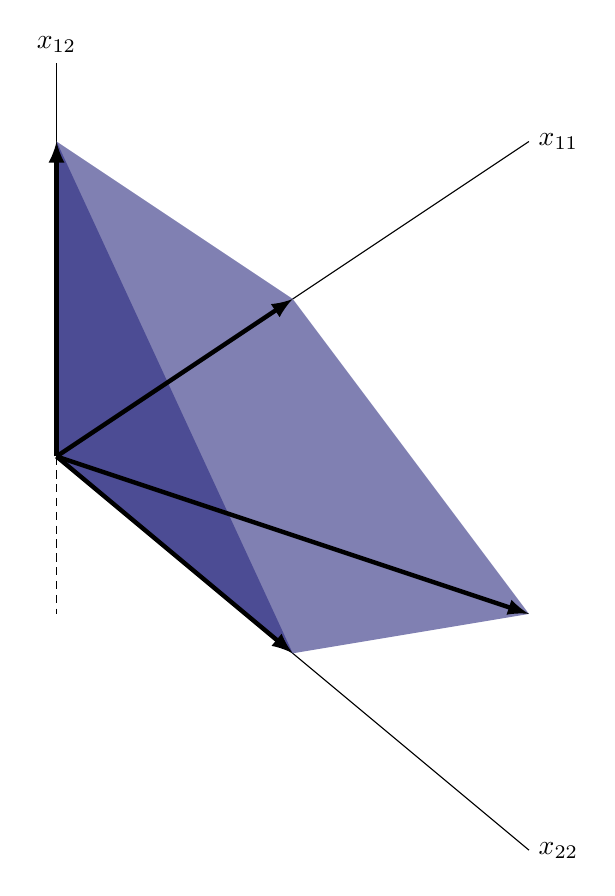
\begin{tikzpicture}[>=latex]
        \draw (0,0) -- (0,5) node [above, black] {$x_{12}$};
        \draw[densely dashed] (0,0) -- (0,-2);
        \draw (0,0) -- (6,-5) node [right, black] {$x_{22}$};
        \draw (0,0) -- (6,4) node [right, black] {$x_{11}$};

        \fill[blue!40!black!50!white] (0,0) -- (3,2) -- (0,4);
        \fill[blue!40!black!50!white] (0,0) -- (3,2) -- (6,-2);
        \fill[blue!40!black!50!white] (0,0) -- (3,-2.5) -- (6,-2);
        \fill[blue!40!black!70!white] (0,0) -- (3,-2.5) -- (0,4);

        \draw [->,ultra thick] (0,0) -- (0,4); 
        \draw [->,ultra thick] (0,0) -- (3,-2.5); 
        \draw [->,ultra thick] (0,0) -- (3,2); 
        \draw [->,ultra thick] (0,0) -- (6,-2); 
    \end{tikzpicture}

    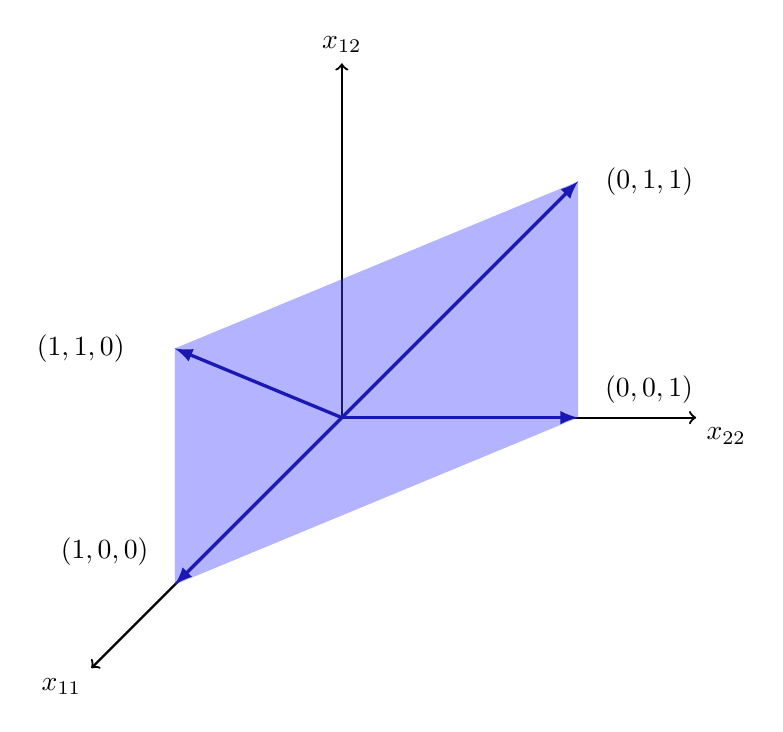
\begin{tikzpicture}%
        [x={(-0.707106cm, -0.707106cm)},
        y={(1cm, 0cm)},
        z={(0cm, 1cm)},
        scale=3.000000,
        back/.style={loosely dotted, thin},
        edge/.style={color=blue!50!black, very thick},
        facet/.style={fill=blue!75!white,fill opacity=0.400000},
        vertex/.style={inner sep=1pt,circle,draw=blue!50!black,fill=blue!50!black,thick}]

    %% Drawing the axes
    \draw[color=black,thick,->] (0,0,0) -- (1.5,0,0) node[anchor=north east]{$x_{11}$};
    \draw[color=black,thick,->] (0,0,0) -- (0,1.5,0) node[anchor=north west]{$x_{22}$};
    \draw[color=black,thick,->] (0,0,0) -- (0,0,1.5) node[anchor=south]{$x_{12}$};
    %% Rays for cone:   
    \draw[color=blue!50!black,very thick,-latex] (0,0,0)--(1,0,1);
    \draw[color=blue!50!black,very thick,-latex] (0,0,0)--(0,1,0);
    \draw[color=blue!50!black,very thick,-latex] (0,0,0)--(1,0,0);
    \draw[color=blue!50!black,very thick,-latex] (0,0,0)--(0,1,1);
    %%
    %% Drawing the interior
    %%
    \fill[facet] (0, 0, 0) -- (0, 1, 0) -- (0, 1, 1) -- (0, 0, 0) -- cycle {};
    \fill[facet] (0,0,0) -- (0, 1, 1) -- (1, 0, 1) -- (0, 0, 0) -- cycle {};
    \fill[facet] (0,0,0) -- (1,0,1) -- (1, 0, 0) -- (0, 0, 0) -- cycle {};
    \fill[facet] (0, 0, 0) -- (1, 0, 0) -- (0, 1, 0) -- (0, 0, 0) -- cycle {};
    %%
    %% Drawing the vertices
    %%
    \node[label={[label distance=0.1cm]0:$(0,1,1)$}] at (0.00000, 1.00000, 1.00000)    {};
    \node[label={[label distance=0.1cm]15:$(0,0,1)$}] at (0.00000, 1.00000, 0.00000)     {};
    \node[label={[label distance=0.1cm]150:$(1,0,0)$}] at (1.00000, 0.00000, 0.00000)     {};
    \node[label={[label distance=-2cm]0:$(1,1,0)$}] at (1.00000, 0.00000, 1.00000)     {};
    %%
    %%
    \end{tikzpicture}

    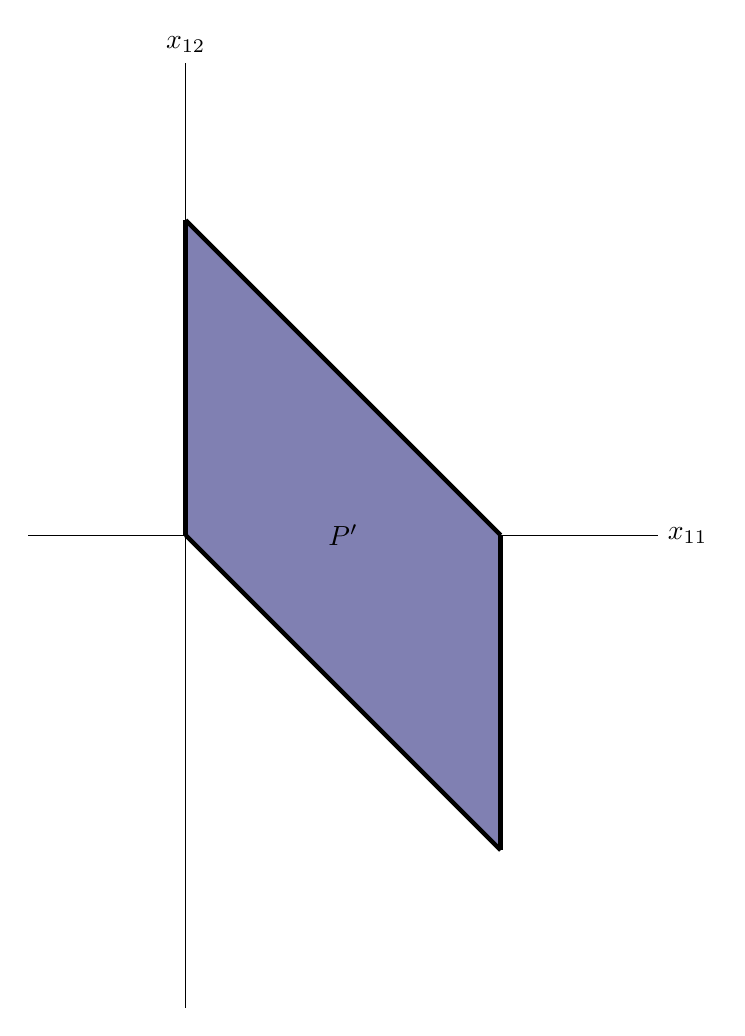
\begin{tikzpicture}
        \draw (-2,0) -- (6,0) node [right, black] {$x_{11}$};
        \draw (0,-6) -- (0,6) node [above, black] {$x_{12}$};

        \fill[blue!40!black!50!white] (0,0) -- (4,-4) -- (4,0) -- (0,4);
        \node at (2,0) {$P^{\prime}$};

        \draw [ultra thick] (0,0) -- (0,4);
        \draw [ultra thick] (0,0) -- (4,-4);
        \draw [ultra thick] (4,-4) -- (4,0);
        \draw [ultra thick] (4,0) -- (0,4);
    \end{tikzpicture}

    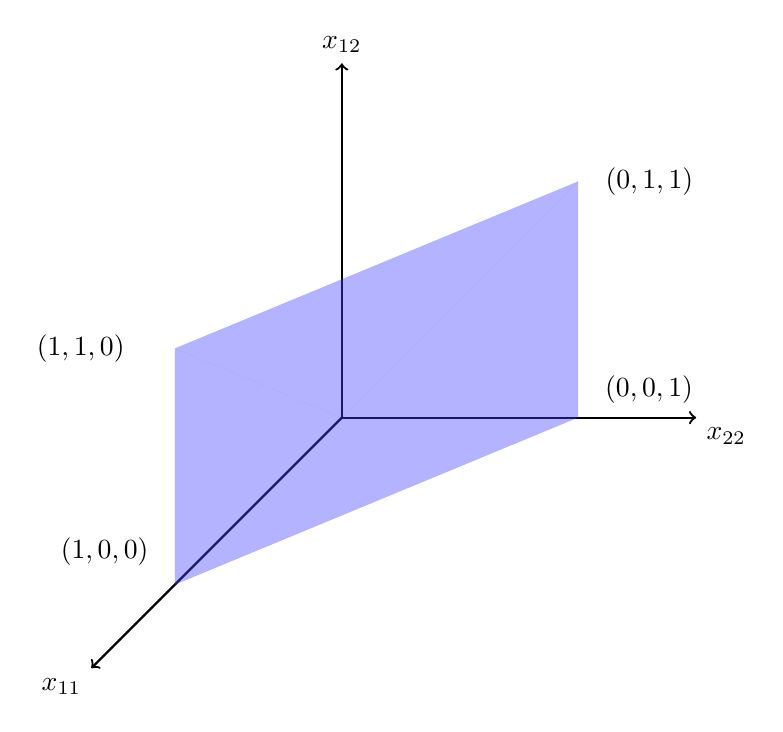
\begin{tikzpicture}%
        [x={(-0.707106cm, -0.707106cm)},
        y={(1cm, 0cm)},
        z={(0cm, 1cm)},
        scale=3.000000,
        back/.style={loosely dotted, thin},
        edge/.style={color=blue!50!black, very thick},
        facet/.style={fill=blue!75!white,fill opacity=0.400000},
        vertex/.style={inner sep=1pt,circle,draw=blue!50!black,fill=blue!50!black,thick}]

    %% Drawing the axes
    \draw[color=black,thick,->] (0,0,0) -- (1.5,0,0) node[anchor=north east]{$x_{11}$};
    \draw[color=black,thick,->] (0,0,0) -- (0,1.5,0) node[anchor=north west]{$x_{22}$};
    \draw[color=black,thick,->] (0,0,0) -- (0,0,1.5) node[anchor=south]{$x_{12}$};
    
    %%
    %% Drawing the interior
    %%
    \fill[facet] (0, 0, 0) -- (0, 1, 0) -- (0, 1, 1) -- (0, 0, 0) -- cycle {};
    \fill[facet] (0,0,0) -- (0, 1, 1) -- (1, 0, 1) -- (0, 0, 0) -- cycle {};
    \fill[facet] (0,0,0) -- (1,0,1) -- (1, 0, 0) -- (0, 0, 0) -- cycle {};
    \fill[facet] (0, 0, 0) -- (1, 0, 0) -- (0, 1, 0) -- (0, 0, 0) -- cycle {};
    %%
    %% Drawing the vertices
    %%
    \node[label={[label distance=0.1cm]0:$(0,1,1)$}] at (0.00000, 1.00000, 1.00000)    {};
    \node[label={[label distance=0.1cm]15:$(0,0,1)$}] at (0.00000, 1.00000, 0.00000)     {};
    \node[label={[label distance=0.1cm]150:$(1,0,0)$}] at (1.00000, 0.00000, 0.00000)     {};
    \node[label={[label distance=-2cm]0:$(1,1,0)$}] at (1.00000, 0.00000, 1.00000)     {};
    %%
    %%
    \end{tikzpicture}
    \newpage
    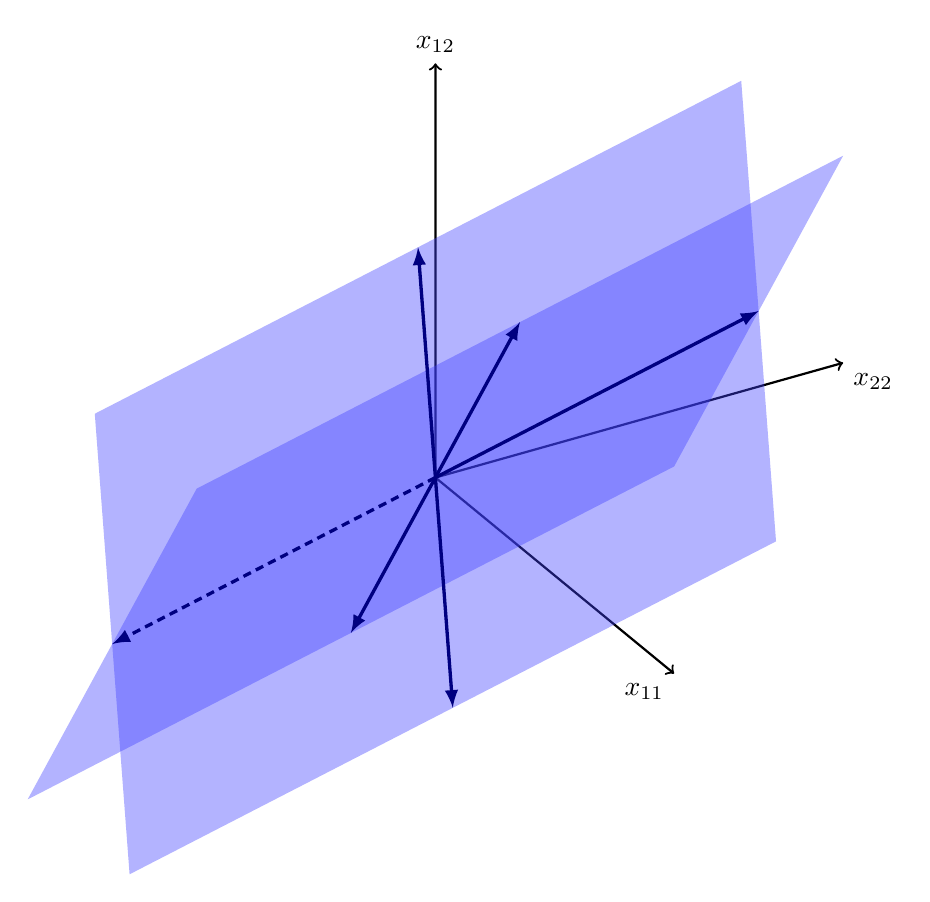
\begin{tikzpicture}%
        %[x={(0.613395cm, -0.260433cm)},
	    %y={(0.782463cm, 0.328575cm)},
	    %z={(-0.107230cm, 0.907862cm)},
        %[x={(0.800797cm, -0.258060cm)},
        %y={(0.598547cm, 0.312295cm)},
        %z={(0.021580cm, 0.914263cm)},
        [x={(0.505216cm, -0.414953cm)},
        y={(0.862993cm, 0.242833cm)},
        z={(0.000089cm, 0.876839cm)},
        scale=3.000000,
        back/.style={loosely dotted, thin},
        edge/.style={color=blue!50!black, thick},
        facet1/.style={fill=blue!75!white,fill opacity=0.400000},
        facet12/.style={fill=blue!75!black,fill opacity=0.400000},
        vertex/.style={inner sep=1pt,circle,draw=black!25!black,fill=black!75!black,thick}]
    %
    %
    %% This TikZ-picture was produced with Sagemath version 9.6
    %% with the command: ._tikz_2d_in_3d and parameters:
    %% view = [-0.567900000000000, -0.474900000000000, -0.672300000000000]
    %% angle = 102.410000000000
    %% scale = 2
    %% edge_color = blue!50!black
    %% facet_color = blue!75!black
    %% opacity = 0.400000000000000
    %% vertex_color = black
    %% axis = True
    
    %% Drawing the axes
    \draw[color=black,thick,->] (0,0,0) -- (2,0,0) node[anchor=north east]{$x_{11}$};
    \draw[color=black,thick,->] (0,0,0) -- (0,2,0) node[anchor=north west]{$x_{22}$};
    \draw[color=black,thick,->] (0,0,0) -- (0,0,2) node[anchor=south]{$x_{12}$};
    %%
    %% Drawing the interior
    %%
    \fill[facet1] (0, 0, 0) -- (1,-0.5,-0.5) -- (0,-1.5,-1.5) -- (-1,-1,-1) -- (0, 0, 0) -- cycle {};
    \fill[facet1] (0, 0, 0) -- (1,-1,0) -- (0,-2,-1) -- (-1,-1,-1) -- (0, 0, 0) -- cycle {};
    \fill[facet1] (0, 0, 0) -- (1,-0.5,-0.5) -- (2,0.5,0.5) -- (1,1,1) -- (0, 0, 0) -- cycle {};
    \fill[facet1] (0, 0, 0) -- (1,-1,0) -- (2,0,1) -- (1,1,1) -- (0, 0, 0) -- cycle {};
    \fill[facet1] (0, 0, 0) -- (-1,0.5,0.5) -- (-2,-0.5,-0.5) -- (-1,-1,-1) -- (0, 0, 0) -- cycle {};
    \fill[facet1] (0, 0, 0) -- (-1,0.5,0.5) -- (0,1.5,1.5) -- (1,1,1) -- (0, 0, 0) -- cycle {};
    \fill[facet1] (0, 0, 0) -- (-1,1,0) -- (-2,0,-1) -- (-1,-1,-1) -- (0, 0, 0) -- cycle {};
    \fill[facet1] (0, 0, 0) -- (-1,1,0) -- (0,2,1) -- (1,1,1) -- (0, 0, 0) -- cycle {};
    
    %% Rays for normal cones:   
    \draw[color=blue!50!black,very thick,-latex] (0,0,0)--(1,-0.5,-0.5);
    \draw[color=blue!50!black,very thick,-latex] (0,0,0)--(1,-1,0);
    \draw[color=blue!50!black,very thick,-latex] (0,0,0)--(-1,1,0);
    \draw[color=blue!50!black,very thick,-latex] (0,0,0)--(-1,0.5,0.5);
    \draw[color=blue!50!black,very thick,-latex] (0,0,0)--(1,1,1);
    \draw[densely dashed, color=blue!50!black,very thick,-latex] (0,0,0)--(-1,-1,-1);
    %% Drawing the vertices
    %%
    %\node[label={[label distance=0.1cm]0:$(0,1,1)$}] at (0.00000, 1.00000, 1.00000)    {};
    %\node[label={[label distance=0.1cm]15:$(0,0,1)$}] at (0.00000, 1.00000, 0.00000)     {};
    %\node[label={[label distance=0.1cm]150:$(1,0,0)$}] at (1.00000, 0.00000, 0.00000)     {};
    %\node[label={[label distance=-2cm]0:$(1,1,0)$}] at (1.00000, 0.00000, 1.00000)     {};
    %%
    %%
    \end{tikzpicture}
\end{document}